\documentclass[aspectratio=169]{beamer}

\usepackage[utf8]{inputenx} % For æ, ø, å
\usepackage{csquotes}       % Quotation marks
\usepackage{microtype}      % Improved typography
\usepackage{amssymb}        % Mathematical symbols
\usepackage{mathtools}      % Mathematical symbols
\usepackage[absolute, overlay]{textpos} % Arbitrary placement
\setlength{\TPHorizModule}{\paperwidth} % Textpos units
\setlength{\TPVertModule}{\paperheight} % Textpos units
\usepackage{tikz}
\usetikzlibrary{overlay-beamer-styles}  % Overlay effects for TikZ

\AtBeginSection{\frame{\sectionpage}}
\AtBeginSubsection{\frame{\subsectionpage}}

\usepackage{hyperref}
\usepackage{svg}
%\usefonttheme{serif}

\usepackage{xfrac}
\usepackage{color, soul, xcolor} % Colored text and highlighting, respectively
\makeatletter
\let\HL\hl
\renewcommand\hl{%
  \let\set@color\beamerorig@set@color
  \let\reset@color\beamerorig@reset@color
  \HL}
\makeatother
\usepackage{tikz-cd} % For commutative diagrams
\usepackage{tikz-3dplot}
\usetikzlibrary{angles}
\RequirePackage{pgfplots}
\usepackage{mathtools}
\usepackage{answers}
\usepackage{setspace}
\usepackage{graphicx}
\usepackage{enumerate}
\usepackage{multicol}
\usepackage{mathrsfs}
\usepackage{amsmath,amsthm,amssymb}
\usepackage{marvosym,wasysym} %fucking smileys
\usepackage{float}
\usepackage{morefloats}
\usepackage{pgf,tikz}
\pgfplotsset{compat=1.15}
\usepackage{mathrsfs}
\usetikzlibrary{arrows}
\usepackage{subcaption}
\usepackage[most]{tcolorbox}
\tcbuselibrary{theorems}
\usepackage{fancyvrb}
\usepackage{longtable,booktabs}
\usepackage{stackrel}
\usepackage{animate}
\usepackage[percent]{overpic}
\definecolor{lighter_csu_green}{RGB}{60,133,77}
\newcommand\boldgreen[1]{\textcolor{lighter_csu_green}{\emph{\textbf{#1}}}}
\usepackage{MnSymbol}
%border matrix
\makeatletter
\newif\if@borderstar
\def\bordermatrix{\@ifnextchar*{%
\@borderstartrue\@bordermatrix@i}{\@borderstarfalse\@bordermatrix@i*}%
}
\def\@bordermatrix@i*{\@ifnextchar[{\@bordermatrix@ii}{\@bordermatrix@ii[()]}}
\def\@bordermatrix@ii[#1]#2{%
\begingroup
\m@th\@tempdima8.75\p@\setbox\z@\vbox{%
\def\cr{\crcr\noalign{\kern 2\p@\global\let\cr\endline }}%
\ialign {$##$\hfil\kern 2\p@\kern\@tempdima & \thinspace %
\hfil $##$\hfil && \quad\hfil $##$\hfil\crcr\omit\strut %
\hfil\crcr\noalign{\kern -\baselineskip}#2\crcr\omit %
\strut\cr}}%
\setbox\tw@\vbox{\unvcopy\z@\global\setbox\@ne\lastbox}%
\setbox\tw@\hbox{\unhbox\@ne\unskip\global\setbox\@ne\lastbox}%
\setbox\tw@\hbox{%
$\kern\wd\@ne\kern -\@tempdima\left\@firstoftwo#1%
\if@borderstar\kern2pt\else\kern -\wd\@ne\fi%
\global\setbox\@ne\vbox{\box\@ne\if@borderstar\else\kern 2\p@\fi}%
\vcenter{\if@borderstar\else\kern -\ht\@ne\fi%
\unvbox\z@\kern-\if@borderstar2\fi\baselineskip}%
\if@borderstar\kern-2\@tempdima\kern2\p@\else\,\fi\right\@secondoftwo#1 $%
}\null \;\vbox{\kern\ht\@ne\box\tw@}%
\endgroup
}
\makeatother

\usetheme{UiB}

%For easier reading
\setbeamersize{text margin left=40pt,text margin right=40pt}
\renewcommand{\baselinestretch}{1.3}


%% FONT STUFF
\usepackage{amsmath}
\usepackage{amsfonts}
\usefonttheme[onlymath]{serif}

%Commands
\newcommand{\R}{\mathbb{R}}
\newcommand{\C}{\mathbb{C}}
\newcommand{\opens}{\mathcal{O}}
\newcommand{\hilbert}{\mathcal{H}}
\newcommand{\algebra}{\mathcal{A}}
\newcommand{\ideals}{\mathcal{I}}
\newcommand{\functionals}{\mathcal{M}}
\newcommand{\spec}{\mathrm{spec}}
\newcommand{\clifford}{\mathrm{C}\ell}
    \newcommand\quotient[2]{
        \mathchoice
            {% \displaystyle
                \text{\raise1ex\hbox{$#1$}\Big/\lower1ex\hbox{$#2$}}%
            }
            {% \textstyle
                #1\,/\,#2
            }
            {% \scriptstyle
                #1\,/\,#2
            }
            {% \scriptscriptstyle  
                #1\,/\,#2
            }
    }


\author{Colin Roberts}
\setbeamercolor{title}{fg=white} 
\title{The Calder\'on Problem}
\setbeamercolor{subtitle}{fg=white} 
\subtitle{on Riemannian Manifolds}



\begin{document}

\begin{frame}{Outline}
\vfill
    \begin{itemize}
    \pause
        \item Introduce the Calder\'on problem.
        
        \pause
        \item Discuss some of the current results and issues.
        
        \pause
        \item Rephrase the problem in a geometrical way.
        
        \pause
        \item Prove the problem in 2 dimensions using the boundary control method.
        
        \pause
        \item What can and can't we do to generalize this method?
    \end{itemize}
\vfill    
\end{frame}

\section{Introduction}

\subsection{Calder\'on Problem}

\begin{frame}{}
\vfill
In 1980, Alberto Calder\'on proposed a problem in his paper \emph{On an inverse boundary value problem}. 
\pause
    \begin{itemize}
        \item He wanted to know if one can determine the conductivity of a domain by making voltage and current measurements along the boundary.
        
        \pause
        \item This is the Electrical Impedence Tomography problem.
        
        \pause
        \item Originally his motivation was for oil prospecting. 
        
        \pause
        \item This problem sparked interest due to its usefulness in geophysical and medical imaging.
    \end{itemize}
\vfill
\end{frame}

\begin{frame}{}
\vfill
\begin{figure}[H]
    \centering
    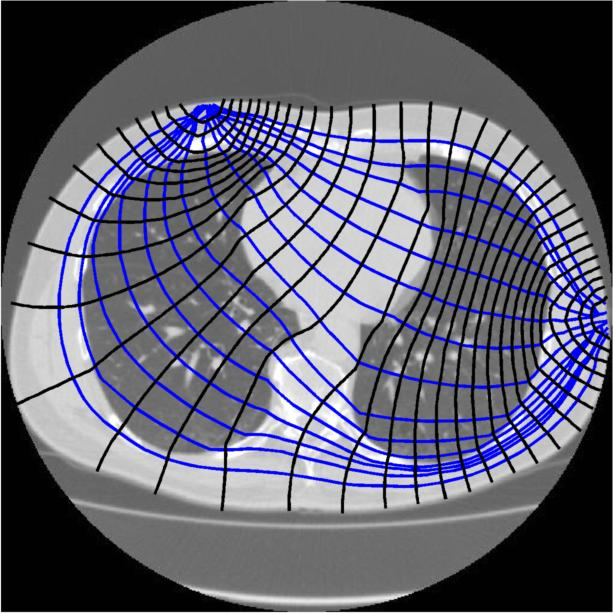
\includegraphics[width=.5\textwidth]{eit.jpg}
\end{figure}
\vfill
\end{frame}

\begin{frame}{}
\vfill
The two main groups working on this problem now are... 
\pause
    \begin{itemize}
        \item Practitioners: Work with incomplete and noisy data to recover information in the real world.
        
        \pause
        \item Theorists: Work in ideal scenarios with a chosen amount of information to see the scope of possibilities.
    \end{itemize}
\vfill    
\end{frame}

\begin{frame}{}
\vfill
The two main groups working on this problem now are... 
    \begin{itemize}
        \item Practitioners: Work with incomplete and noisy data to recover information in the real world.
        
        \item \hl{Theorists: Work in ideal scenarios with a chosen amount of information to see the scope of possibilities.}
    \end{itemize}
\vfill
\end{frame}

\begin{frame}{Problem Statement}
\vfill
    \textbf{\underline{Idea:}} Given a domain $\Omega$ with interior $\Omega^+$ that we cannot probe, can we determine the conductivity $\gamma$ matrix by studying the boundary $\partial \Omega$? 
    \pause
    \begin{itemize}
        \item $\Omega^+$ is free of charges, hence $\nabla \cdot (\gamma \nabla u) = 0$ in $\Omega^+$ where $u$ is the electrostatic potential.
        
        \pause
        \item Apply a known voltage $f$ at the boundary $\partial \Omega$. Hence $f = u \vert_{\partial \Omega}$.
        
        \pause
        \item Measure the current flux $h$ through the boundary $\partial \Omega$. Hence, $h = \frac{\partial u}{\partial \nu}$.
        
        \pause
        \item This defines the voltage-to-current map $\Lambda$ so that $\Lambda(f) = h$.
        
        \pause
        \item Can we determine the conductivity matrix $\gamma$ from $\Lambda$?
    \end{itemize}
\vfill
\end{frame}


\section{The Calder\'on Problem on Riemannian Manifolds}

\subsection{Preliminaries}

\begin{frame}{Geometry}
\vfill
    \pause
    \begin{itemize}
        \item \boldgreen{Smooth $n$-dimensional manifold}: A space that locally looks like (is $C^\infty$ diffeomorphic to) an open subset of $\R^n$.
        
        \pause 
        \item \boldgreen{Riemannian metric}: A smoothly varying inner product defined on $\Omega$.  In coordinates, $g$ takes the form of a symmetric and positive definite matrix with entries $g_{jk}$ with inverse $g^{jk}$.
        
        \pause
        \item \boldgreen{Exterior algebra}: Differential forms with the wedge product $\wedge$.
        
        \pause
        \item \boldgreen{Hodge Star}: Attached to the exterior algebra when we also have a Riemannian metric.  Gives an isomorphism between $k$ and $n-k$-forms.
    \end{itemize}
\vfill
\end{frame}

\begin{frame}{}
\vfill
\begin{figure}[H]
	\centering
	\def\svgwidth{.9\columnwidth}
	\input{sphere_charts_maps.pdf_tex}
\end{figure}
\vfill
\end{frame}

\begin{frame}{}
\vfill
\begin{figure}[H]
	\centering
	\def\svgwidth{\columnwidth}
	\input{pushforward.pdf_tex}
\end{figure}
\vfill
\end{frame}

\begin{frame}{}
\begin{figure}[H]
	\hspace*{-2cm}
	\def\svgwidth{1.2\columnwidth}
	\input{area.pdf_tex}
\end{figure}
\vfill
\end{frame}

\begin{frame}{1-Forms}
\begin{figure}[H]
    \centering
	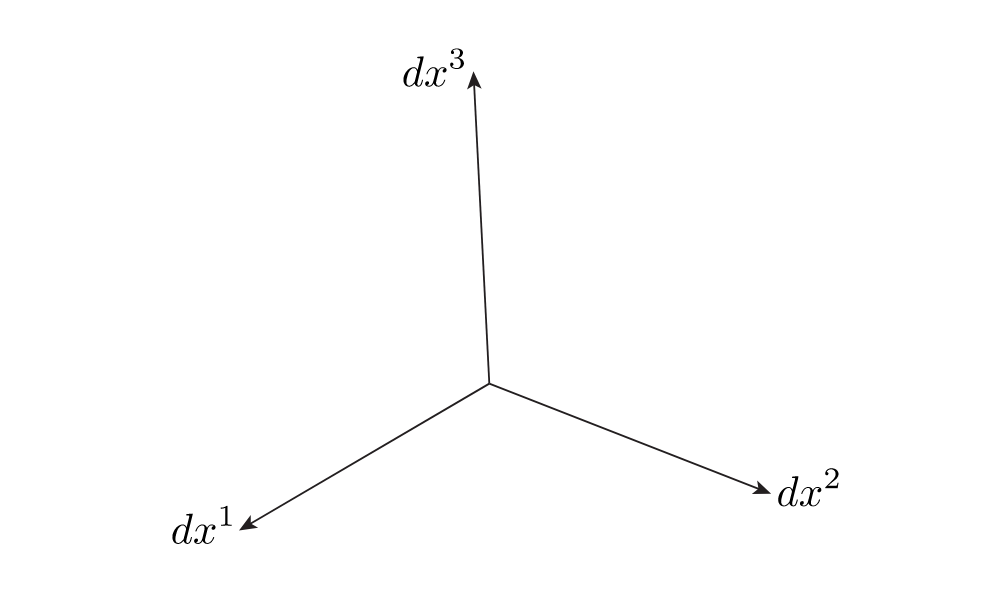
\includegraphics[width=.8\columnwidth]{1forms.png}
\end{figure}
\vfill
\end{frame}

\begin{frame}{2-Forms}
\begin{figure}[H]
    \centering
	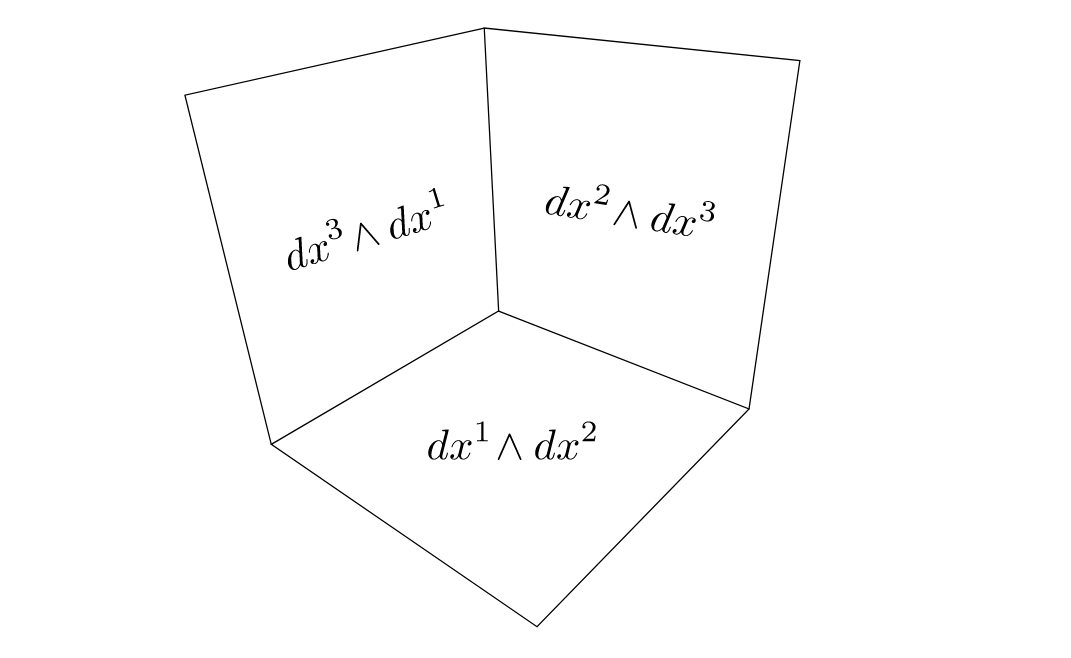
\includegraphics[width=.8\columnwidth]{2forms.png}
\end{figure}
\vfill
\end{frame}

\begin{frame}{3-Forms}
\vfill
\begin{figure}[H]
    \centering
	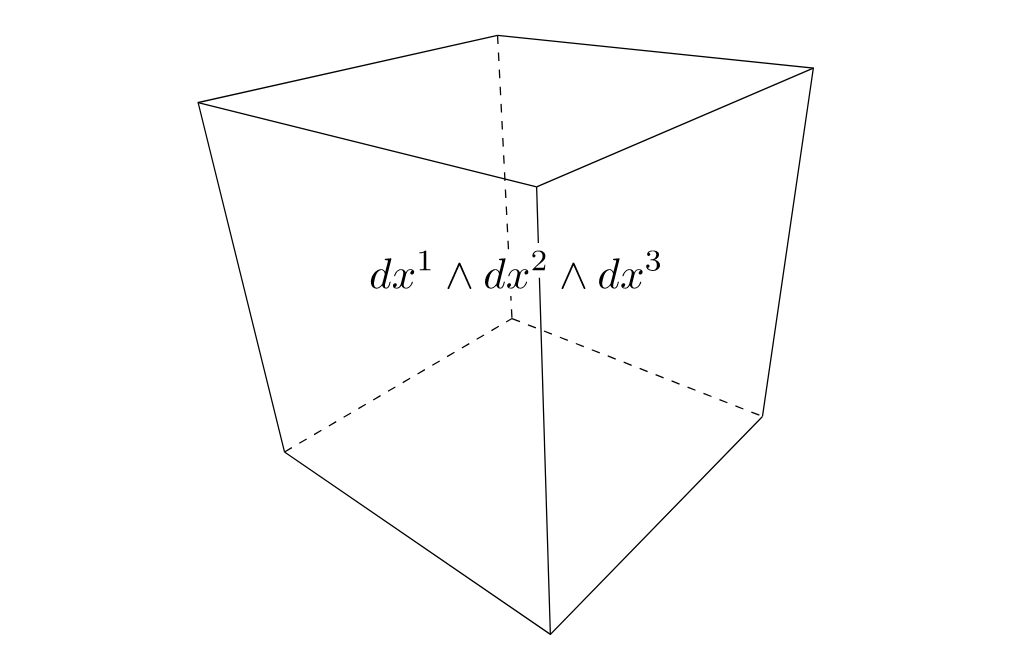
\includegraphics[width=.8\columnwidth]{3forms.png}
\end{figure}
\vfill
\end{frame}




\begin{frame}{Partial Differential Equations}
    \vfill
    \pause
    \begin{itemize} 
    \item \boldgreen{$k$-Form Inner Product}: $\displaystyle{\langle\alpha,\beta\rangle = \int_\Omega \alpha \wedge \star \beta}$.
    \pause
    
        \item \boldgreen{Exterior Derivative}: Derivative operator $d$ defined on $k$-forms.  
        
        \pause 
        \item \boldgreen{Codifferential}: Formal adjoint to $d$ written as $\delta$.
        
        \pause
        \item \boldgreen{Dirac Operator}: $D=d+\delta$.
        
        \pause
        \item \boldgreen{Laplace-Beltrami Operator}: $\Delta = d\delta +\delta d=D^2$ and in coordinates
        \[
        \Delta f = \frac{1}{\sqrt{|g|}} \sum_{j=1}^n \sum_{k=1}^n \frac{\partial}{\partial x^i} \sqrt{|g|} g^{ij} \frac{\partial}{\partial x^j} f 
        \]
    \end{itemize}
\end{frame}

\subsection{Raphrasing EIT Problem in a Geometrical Language}

\begin{frame}{}
\vfill 
    \begin{itemize}
        \pause
        \item Let (unknown) connected $\Omega$ be a smooth Riemannian manifold with boundary $\partial \Omega$.
        
        \pause
        \item Replace conductivity be represented by (unknown) $g$ since $\gamma^{jk}=\sqrt{|g|}g^{jk}$.
        
        \pause
        \item Let $\Delta u = 0$ in $\Omega^+$ and $u=f$ on $\partial \Omega$.
        
        \pause
        \item \boldgreen{Dirichlet-to-Neumann operator} $\Lambda$ maps Dirichlet data $f=u|_{\partial \Omega}$ to $g = \frac{\partial u}{\partial \nu}=\iota^*(\star d u)$.
        
        \pause
        \item Recover $g$ from knowing $\Lambda$.
    
    \end{itemize}
\end{frame}

\subsection{Expected and Current Results}

\begin{frame}{Formal Variable Count}
    \pause $f \mapsto \Lambda(f)$ approximated by
    \[
    \Lambda(f)_j = \sum_{k=1}^m \lambda_{jk} f_k.
    \]
    
    \pause In the smooth setting,
    \[
    \Lambda(f) = \int_{\partial \Omega} \lambda(x,y) f(y)dS(y).
    \]
    
    \pause So, $g$ is a function of $n$ variables that needs to be determined by the kernel $\lambda$ which is $2n-2$ variables.
\end{frame}

\begin{frame}{Formal Variable Count}
\vfill
\begin{itemize}
    \pause 
    \item $n=1$ gives us an undetermined system.
    
    \pause
    \item $n=2$ is well determined.
    
    \pause
    \item $n\geq 3$ is overdetermined.
   \end{itemize}
\vfill   
\end{frame}

\begin{frame}{Issue In 2-Dimensions}
    \pause In 2D, $\Delta$ is conformally invariant.  \\
    
    \vspace*{.5cm}
    \pause Indeed, let $\tilde{g}=e^{2\phi}g$, then
    \[
    \Delta_{\tilde{g}} = e^{-2\phi}\Delta_g +(n-2)e^{-2\phi} g^{jk} \frac{\partial \phi}{\partial x^k} \frac{\partial}{\partial x^j}
    \]
    
    \pause When $n=2$, the extra term cancels.
\end{frame}

\begin{frame}{1 Dimension}
\vfill
\pause
    \begin{itemize}
        \item The problem in 1 dimension is trivial.
        
        \pause
        \item Can only know the total impedence between the two electrodes.
        
    \end{itemize}
\vfill
\end{frame}

\begin{frame}{Isotropic Case}
    For $g$ isotropic and $n\geq 3$ one can determine $g$ from $\Lambda$. \\
    (\emph{Sylvester-Uhlmann 1987})
    
\end{frame}

\begin{frame}{2 Dimensional Anisotropic}
\vfill
    \begin{itemize}
        \item Can recover $g$ up to conformal class and can't do better.
        \item Proven by Lassas and Uhlmann in \emph{On Determining the Riemannian manifold from the Dirichlet to Neumann map}.
    \end{itemize}
\vfill
\end{frame}

\begin{frame}{3+ Dimensional Anisotropic}
\vfill
\pause
    \begin{itemize}
        \item For real analytic manifolds, the (scalar/classical) DN map determines the manifold up to isometry.  This gives the topological information as well. (Lassas, Taylor, Uhlmann \emph{The Dirichlet-to-Neumann map for complete Riemannian manifolds with boundary}.
        
        \pause
        \item Can determine the boundary $C^\infty$-jet of $g$ in Lee and Uhlmann's \emph{Determining anisotropic real-analytic conductivities by boundary measurements.}
        
        \pause
        \item For smooth manifolds, the anisotropic problem is open. The goal is to recover the metric up to isometry.
    \end{itemize}
\end{frame}



\section{Boundary Control Method in 2 Dimensions}

\begin{frame}{Theorem}
    \pause
    \emph{Two $2$-dimensional compact orientable manifolds with single common boundary are conformally equivalent iff their DN-maps coincide.}\\
    
    \vspace*{1cm}
    Belishev's \emph{The Calder\'on Problem for Two-Dimensional Manifolds by the BC-Method.}
\end{frame}


\begin{frame}{Key Ideas}
\vfill
\pause
    \begin{itemize}
        \item Surfaces are two dimensional and can be related to $\C$.
        
        \pause
        \item Holomorphic functions have components that are harmonic.
        
        \pause
        \item Hilbert transform converts one harmonic function to another by connecting them via a single holomorphic function.
        
        \pause
        \item Gelfand transform relates an algebra $\algebra$ to the algebra of continuous functions on the spectrum of that algebra, $C(\spec \algebra)$.
        
        \pause
        \item This gives us a way to realize $\Omega$ from functions defined on $\Omega$ that we have access to.
    \end{itemize}
\vfill
\end{frame}

\begin{frame}{Outline of the Proof}
\vfill
\pause
    \begin{itemize}
        \item From DN map, recover the algebra of holomorphic functions. (Lemma 1)
        
        \pause
        \item Show that this algebra is generic. (Lemma 2)
        
        \pause
        \item Represent the trace algebra with the DN map. (Lemma 3)
        
        \pause
        \item Construct the manifold. (Theorem)
    \end{itemize}
\vfill
\end{frame}

\begin{frame}{Some Notes}
    \vfill
    \begin{itemize}
    \pause
    \item We have the inclusion of the boundary $\iota \colon \partial \Omega \to \Omega$.
    
    \pause
    \item The pullback $\iota^* \colon T^*\Omega \to T^*\partial \Omega$.
    
    \pause
    \item Define $\Lambda$ by $\iota^*(\star d u)$ for a harmonic $u$.
    
    \pause
    \item $\Lambda$ maps boundary $k$-forms to boundary $n-k-1$ forms.
    \end{itemize}
\end{frame}

\begin{frame}{}
\begin{figure}[H]
    \centering
	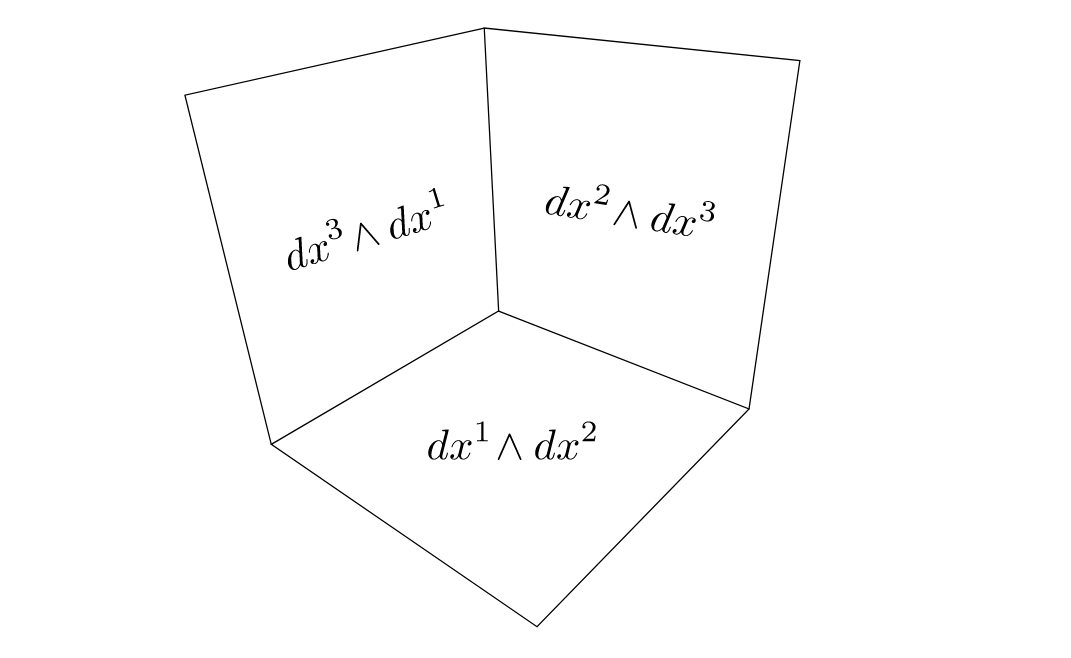
\includegraphics[width=.8\columnwidth]{2forms.png}
\end{figure}
\vfill
\end{frame}

\subsection{Lemma 1}

\begin{frame}{Lemma 1}
\vfill
        \begin{itemize}
            \pause
            \item A function $u$ satisfying $\Delta u =0$ has a conjugate function $v$ if and only if the trace $\iota^* u$ satisfies
            \[
                \left[ \Lambda + d\Lambda^{-1} d\right] \iota^*u = 0.
            \]
            
            \pause
            \item $\dim\textrm{Ran}\left[ \Lambda + d \Lambda^{-1} d \right] = \beta_1(\Omega).$
        \end{itemize}
        \vfill
\end{frame}

\begin{frame}{Corollary}
\vfill
    $\Lambda$ completely determines the topology of $\Omega$.
\vfill
\end{frame}

\begin{frame}{Proof}
\vfill
\pause
    \begin{itemize}
        \item Since $\Omega$ is a single connected component, $\beta_0(\Omega)=1$.
        \item We have $\beta_1(\Omega)$ from before.
        \item Since $\Omega$ is a surface with boundary, $\beta_2(\Omega)=0$.
        \item Since $\Omega$ is two dimensional, $\beta_n(\Omega)=0$ for $n\geq 3$.
    \end{itemize}
\vfill
\end{frame}

\begin{frame}{Conjugate Function Intuition}
\vfill
\begin{itemize}
   \pause
   \item Suppose we have homorphic complex function $w = u + i v$.  
   
   \pause
   \item Let $u$ be a 0-form and $v$ as a 2-form.
   
   \pause
   \item Then $\frac{\partial}{\partial \overline{z}}$ is given by $D=d+\delta$.
   
   \pause
   \item $Dw=0$ gives us the Cauchy-Riemann equations
    
   \item We call $u$ and $v$ conjugate by CREs.    
\end{itemize}
\vfill
\end{frame}

\begin{frame}{Hilbert Transform}
\vfill
\begin{itemize}
    \pause
    \item We can get $v$ from $u$ via the Hilbert transform.
    
    \pause
    \item Define $\hilbert = d \Lambda^{-1}$.
\end{itemize}
\vfill
\end{frame}

\begin{frame}{Construct the Algebra $\algebra(\Omega)$}
\vfill
\begin{itemize}
    \pause
    \item By Lemma 1 we can now create the algebra $\algebra(\Omega)\subset C(\Omega)$ from harmonic functions $u$ with conjugates $v$ by
    \[
    \algebra(\Omega) \coloneqq \{ w = u+iv\}.
    \]
    Algebra since product of two holomorphic functions is holomorphic.
    
    \pause
    \item In isothermal coordinates, each $w\in \algebra(\Omega)$ is holomorphic.
    
    \pause
    \item This gives $\Omega$ a complex structure.
    
    \pause
    \item This is analogous to having the Hodge star on a surface.
\end{itemize}
\vfill
\end{frame}

\subsection{Lemma 2}


\begin{frame}{Gelfand Representation}
\vfill
    \begin{itemize}
    \pause
            \item Let $\functionals$ be the set of multiplicative linear functionals on a commutative Banach algebra $\algebra$.
            
        \pause
        \item The Gelfand transform gives a way of representing an algebra $\algebra$ as a function algebra $\hat{\algebra}$.
        
        \pause
        \item The \boldgreen{Gelfand transform} maps $a\in \algebra$ to a function $\hat{a}$ on $\functionals$ by
        \[
        \hat{a}(\delta) \coloneqq \delta(a), \quad \delta \in \functionals.
        \]
        
        \pause
        \item The \boldgreen{Gelfand topology} is the weakest topology on $\functionals$ in which all $\hat{a}$ are continuous. This makes $\functionals$ compact.
        
        \pause
        \item $\functionals$ with this topology is called the \boldgreen{spectrum} $\spec \algebra$.
    \end{itemize}
\vfill
\end{frame}

\begin{frame}{Generic Algebras}
\vfill
    \begin{itemize}
        \pause
        \item The Gelfand transform $\hat{\algebra}$ is a subalgebra of $C(\spec \algebra)$ and $a\mapsto \hat{a}$ is an isometric isomorphism.
        
%        \pause
%        \item An isomorphism $t\colon A(X) \to B(Y)$ between two function algebras is \boldgreen{spatial} if there exists a bijection $b \colon X \to Y$ such that $tw=w\circ b^{-1}$.  
        
        \pause
        \item For a function algebra $\algebra \subset C(X)$, take $\epsilon \colon X \to \spec \algebra$ with $\epsilon(x)=\delta_x$.
        
        \pause
        \item A function algebra $\algebra \subset C(X)$ is \boldgreen{generic} if $\epsilon$ is a homeomorphism. 
        
        \pause
        \item A generic algebra is (spatially) isomorphic to its Gelfand transform.
        
    \end{itemize}
\vfill
\end{frame}

\begin{frame}{Lemma 2}
\vfill
\pause
    The algebra of holomorphic functions $\algebra(\Omega)$ is generic.
\vfill
\end{frame}

\begin{frame}{Importance}
\vfill
    \begin{itemize}       
        \pause
        \item $\hat{\algebra}(\partial \Omega)$ is (spatially) isomorphic to $\algebra(\Omega)$ by taking the Gelfand transform of the trace.
        
        \pause
        \item The lemma shows that $\epsilon \colon \Omega \to \spec \algebra(\Omega)$ is a homeomorphism, so we have determined $\Omega$ up to homeomorphism.
    \end{itemize}
\vfill
\end{frame}

\begin{frame}{What's Left?}
\vfill
\pause

    We can only have hope access to the trace algebra $\algebra(\partial \Omega)$. So we need to determine this to reach our goal.
    \vfill
\end{frame}

%\begin{frame}{Commutative Banach Algebras (CBA)}
%\vfill
%    \begin{itemize}
%        \pause
%        \item An algebra $\algebra$ is a \boldgreen{commutative Banach Algebra} if 
%        \begin{itemize}
%            \item $\algebra$ is a Banach space.
%            \item $a,b \in \algebra$ satisfy $\|ab\|\leq \|a\|\|b\|$.
%        \end{itemize}
%        
%        \pause
%        \item $\algebra(\Omega) \subset C(\Omega)$.
%        
%        \pause
%        \item $C(\Omega)$ is a CBA and $\algebra(\Omega)$ is a subalgebra.
%        
%        \pause
%        \item $C(\Omega)$ is a \boldgreen{uniform} algebra so $\|a^2\|=\|a\|^2$.
%    \end{itemize}
%\vfill
%\end{frame}
%
%\begin{frame}{Ideals and Functionals}
%\vfill
%    \begin{itemize}
%        \pause
%        \item A subspace $I\neq \algebra$ is an \boldgreen{ideal} if $ja \in I$ for $j\in I$ and $a\in \algebra$.
%        
%        \pause
%        \item An ideal is \boldgreen{maximal} if $\tilde{I}\subset \algebra$ and $I\subset \tilde{I}$ implies $I=\tilde{I}$.
%        
%        \pause 
%        \item A functional $\delta \in \algebra'$ is \boldgreen{multiplicative} if $\delta(ab)=\delta(a)\delta(b)$. 
%        
%        \pause
%        \item Ex: Dirac measure since $\delta_x(ab)=a(x)b(x)$.  
%    \end{itemize}
%\vfill
%\end{frame}

%\begin{frame}{Ideals and Functionals}
%\vfill
%    \begin{itemize}
%        \pause
%        \item Let $\ideals$ be the set of maximal ideals of $\algebra$.
%        
%        \pause
%        \item Let $\functionals$ be the set of multiplicative functions on $\algebra$.
%        
%        \pause
%        \item These sets are in bijection. 
%        
%        \begin{itemize}
%            \item If $\delta \in \functionals$ then $I_\delta \coloneqq \ker \delta \in \ideals$.  
%            \item If $I\in \ideals$ then $\delta_I \colon \algebra \to \algebra / I = \C$ is in $\functionals$.
%        \end{itemize}
%    \end{itemize}
%\vfill
%\end{frame}






\subsection{Lemma 3}

\begin{frame}{Trace Algebra}
\vfill
    \begin{itemize}
        \pause
        \item The trace algebra $\algebra (\partial \Omega) \coloneqq \iota^* \algebra(\Omega)$ is isometrically isomorphic to $\algebra(\Omega)$ since
        \[
        \|w\|_{\algebra(\Omega)} = \|\iota^* w \|_{\algebra(\partial \Omega)}
        \]
        and since a holomorphic function is uniquely determined by its boundary values.
    \end{itemize}
\vfill
\end{frame}

\begin{frame}{Lemma 3}
\vfill
    We have the representation
    \[
    \algebra(\partial \Omega) = \mathrm{clos}_{C(\partial \Omega)} \{ f +i h\},
    \]
    where $h$ is conjugate to $f$ by $\hilbert$.
\vfill
\end{frame}

\subsection{Proof of the Main Theorem}


\begin{frame}{Construction of the Manifold}
\vfill
\pause
Following these steps yields a manifold $(\Omega, g)$ with the DN map $\Lambda$.
    \begin{itemize}
        \pause
        \item \underline{Step 1:} We know $g|_{\partial \Omega}$ by Lee and Uhlmann, and thus we know $\hilbert$ and $C^\infty(\partial \Omega)$.  This allows us to recover the trace algebra $\algebra(\partial \Omega)$ using the representation in Lemma 3.
        
        \pause
        \item \underline{Step 2:} Then find $\spec \algebra(\partial \Omega)=\Omega$ by Lemma 2.
        
        \pause 
        \item \underline{Step 3:} Next, the Gelfand transform $\hat{\algebra}(\partial \Omega)=\algebra(\Omega)$ by Lemma 2.
        
        \pause
        \item \underline{Step 4:} $\algebra(\Omega)$ gives us the complex structure on $\Omega$ by Lemma 1.
        
        \pause
        \item \underline{Step 5:} Equip $\Omega$ with a metric $g$ conforming to this complex structure.
    \end{itemize}
\vfill
\end{frame}




\section{Generalizing This Method}

\begin{frame}{First Issue}
\vfill
\pause
    \begin{itemize}
        \item No complex structure in higher dimensions.
    \end{itemize}
    \vfill
\end{frame}

\begin{frame}{Resolution}
\vfill
\pause
    \begin{itemize}
        \item Use a Clifford algebra/calculus structure to replace $\C$.
        
        \pause
        \item The tools of Clifford analysis allow us to recover a notion of holomorphicity known as \boldgreen{monogenicity}.
        
        \pause
        \item We can recover a similar algebra (Hardy space) of monogenic functions.
    \end{itemize}
\vfill    
\end{frame}

\begin{frame}{Clifford Structure}
\vfill
    A Clifford algebra builds upon the exterior algebra of forms.  Given a quadratic space $(V,Q)$, we have
    \pause
    \begin{itemize}
        \item The quotient of the tensor algebra
        \[
        \clifford(V,Q) =\quotient{\bigoplus_{j=0}^\infty V^{\otimes j}}{\langle v \otimes v - Q(v)\rangle}.
        \]
        
        \pause
        \item If $Q=g$ is an inner product, this yields a geometric product on vectors $u,v \in \clifford(V,g)$
        \[
        uv = g(u,v) + u\wedge v.
        \]
        
        \pause
        \item Geometric product can be extended to multivectors.
    \end{itemize}   
\vfill
\end{frame}

\begin{frame}{Familiar Examples}
\vfill
\pause
We have all seen Clifford algebras before.  Indeed, 
\pause
\begin{itemize}
    \item $\C \cong \clifford(\R,-\cdot)$.
    
    \pause
    \item $\C$ also lives inside of $\clifford(\R^2,\cdot)$ as the even subalgebra. That is,
    \[
    x+iy \iff 1x + e_1 \wedge e_2 y,
    \]
    where $e_1\wedge e_2$ is the bivector (and psuedoscalar).  
    \pause
    \item $\mathbb{H}$ lives inside of $\clifford(\R^3,\cdot)$ as the even subalgebra.
\end{itemize}
\vfill
\end{frame} 

\begin{frame}{Clifford Analysis}
\vfill
\begin{itemize}
\pause

    \item We can replace $d+\delta$ with the Dirac operator $D$
    \[
    D = \sum_{j=1}^n e_j \frac{\partial}{\partial x^j}.
    \]
    
    \pause
    \item $D^2 = \Delta$.
    
    \pause
    \item Elements in the kernel of $D$ are monogenic.
    
    \pause
    \item Monogenic objects in even subalgebra have components that are harmonic.
    
    \pause
    \item There are Cauchy integral and Hilbert transform type operators for $D$ in arbitrary dimension.
    \end{itemize}
    \vfill
\end{frame}

\begin{frame}{Second Issue}
    In dimensions greater than 2, even subalgebra is noncommutative.
    \begin{itemize}
        \pause
        \item The spectral theory for Belishev's solution required a commutative Banach algebra.
        
        \pause
        \item The spectral theory for noncommutative Banach algebras is not as developed.
        
        \pause
        \item There is still work to do here to find some way around this.
    \end{itemize}
\end{frame}

\section{Conclusion}

\begin{frame}{Main Story}
    \begin{itemize}
        \pause
        \item Calder\'on proposed a useful and challenging problem for both theorists and practicioners.
        
        \pause
        \item Advances have been made in both areas.
        
        \pause
        \item Ideal results are still not yet obtained.
    \end{itemize}
\end{frame}

\begin{frame}{Novel Approach}
    \begin{itemize}
        \pause
        \item Belishev solved the 2D problem using the boundary control method.
        
        \pause
        \item It relies heavily on complex analysis and the spectral theory for commutative Banach algebras.
        
        \pause
        \item These issues remain if we try to naively generalize this approach.
    \end{itemize}
\end{frame}

\begin{frame}{New Input}
    \begin{itemize}
        \pause
        \item Clifford algebras and analysis replace the complex structure in arbitrary dimension.
        
        \pause
        \item We can still construct the same algebra of holomorphic functions.
        
        \pause
        \item The relevant algebras are noncommutative for dimensions $\geq$ 3.
        
        \pause
        \item There are possibly other tools at our disposal that may be able to replace the loss of commutivity.
    \end{itemize}
\end{frame}

\begin{frame}{}
    \vfill
    \centering \huge{Thank you!}
    \vfill
\end{frame}


%\section*{Bibliography}
%
%\begin{frame}{References}
%    \begin{itemize}
%        \item \url{http://www.numdam.org/article/SLSEDP_2012-2013____A13_0.pdf}
%        \item Dirichlet to Neumann operator on differential forms
%        \item 2d bc method
%        \item The HIlbert Transform on a smooth closed hypersurface
%    \end{itemize}
%\end{frame}

\end{document}

